\id{МРНТИ \href{https://grnti.ru/?p1=52&p2=47&p3=15}{52.47.15}}{https://doi.org/10.58805/kazutb.v.4.25-590}

\begin{articleheader}

\sectionwithauthors{К.Т.Охапова, Ж.К.Шуханова, В.П.Бондаренко, Г.Ф.Сагитова}{ЖАНУАРЛАР МАЙЛАРЫНЫҢ КОРРОЗИЯҒА ҚАРСЫ ҚАСИЕТТЕРІН ТӘЖІРИБЕЛІК
ЗЕРТТЕУ}

{\bfseries К.Т.Охапова\textsuperscript{\envelope }, Ж.К.Шуханова, В.П.Бондаренко,
Г.Ф.Сагитова}
\end{articleheader}
\begin{affiliation}

М.Әуезов атындағы Оңтүстік Қазақстан университеті, Шымкент қ., Қазақстан

\raggedright {\bfseries \textsuperscript{\envelope }}Корреспондент-автор:
\href{mailto:nuri.maksim82@mail.ru}{\nolinkurl{nuri.maksim82@mail.ru}}
\end{affiliation}

Коррозия процестерін зерттеу және металдарды коррозиядан қорғау әдістері
мен қабаттарын жасау қазіргі таңда өзекті заманауи ғылыми-техникалық
мәселелердің бірі болып табылады. Металлды коррозиядан қорғаудың кең
тараған түрі- өндірістік жағдайларда агрессивті ортамен жанасатын
металлдар мен қорытпалардың коррозия жылдамдығын төмендетуге мүмкіндік
беретін ингибиторларды қолдану. Қазіргі уақытта экологиялық таза
технологияларды пайдалана отырып, металлдар мен қорытпаларды қорғауға
арналған жануарлар майы шикізаты негізіндегі қол жетімді, улы емес және
арзан коррозия ингибиторларын жасау «табиғи» химия саласындағы жетекші
тенденциялардың бірі болып табылады.

Бұл жұмыста 1,0 моль/л агрессивті ортада СТ3 көміртекті болатқа жануар
майының коррозияға қарсы тиімділігі гравиметриялық әдіспен зерттелді.
Агрессивті орта ретінде тұзды және қышқылды ерітінділер алынған.
Ингибитордың тиімділігі қалыпты стандартты орта жағдайында 0,5-2,0 г/л
мөлшерінде зерттелген. Болат пластиналарының әртүрлі агрессивті ортада
массасының жоғалуын негізге алып, жалпы 1 жылда кететін массалық шығынды
есептей отырып, жануар майы қосылған ерітіндінің болат пластинасының
коррозияға қарсы көрсеткішінің проценттік тиімділігі анықталды. Жоғары
тиімділікке болат пластина бетіндегі ингибитордың өздігінен
физиосорбциялануы есебінен қол жеткізілетіндігі жатады. Нәтижесінде
жануар майы болат пластиналарының бетінде жылтыр қорғаныс қабатын түзіп,
оның массасының жоғалуына кедергі келтіретіндігі айқындалды. Сонымен
қатар ингибитор концентрациясының жоғарылауы оның коррозияға қарсы
тиімділігінің артуына алып келетіндігін анықтадық.

{\bfseries Түйін сөздер:} ингибитор, коррозия, коррозия жылдамдығы,
бұрғылау ерітіндісі, металдар, жануарлар майы, табиғи ингибиторлар.
\begin{articleheader}

{\bfseries ЭКСПЕРИМЕНТАЛЬНОЕ ИССЛЕДОВАНИЕ АНТИКОРРОЗИОННЫХ СВОЙСТВ ЖИВОТНЫХ ЖИРОВ}

{\bfseries К.Т.Охапова\textsuperscript{\envelope }, Ж.К.Шуханова, В.П.Бондаренко,
Г.Ф.Сагитова}
\end{articleheader}

\begin{affiliation}

Южно-Казахстанский университет им. М. Ауэзова, Шымкент, Казахстан,

e-mail:\href{mailto:nuri.maksim82@mail.ru}{\nolinkurl{nuri.maksim82@mail.ru}}
\end{affiliation}

Исследование коррозионных процессов, разработка методов защиты металлов
от коррозии относятся к актуальным современным научно-техническим
проблемам. Распространенным видом защиты от коррозии металлов является
применение ингибиторов, позволяющих снизить скорость коррозии металлов и
сплавов при контакте с агрессивными средами в промышленных условиях. В
настоящее время создание доступных, нетоксичных и недорогих ингибиторов
коррозии на основе животного сырья для защиты металлов и сплавов с
использованием экологически чистых технологий является одним из ведущих
направлений в области «природной» химии.

В данной работе гравиметрическим методом исследована антикоррозионная
эффективность животного жира к углеродистой стали СТ3 в агрессивной
среде концентрацией 1,0 моль/л. В качестве агрессивной среды были
получены чистые и кислые растворы. Эффективность ингибитора изучали в
количестве 0,5-2,0 г/л при нормальных стандартных условиях окружающей
среды. На основании потери массы стальных пластин в различных
агрессивных средах и расчета общей потери массы за 1 год определена
процентная эффективность показателя антикоррозионной защиты стальных
пластин в растворе с животным жиром. Установлено, что высокая
эффективность достигается за счет физиосорбции ингибитора на поверхности
стальной пластины. В результате установлено, что животный жир создает на
поверхности стальных пластин глянцевый защитный слой, препятствующий
потере их массы. В то же время увеличение концентрации ингибитора
показало повышение антикоррозионной эффективности.

{\bfseries Ключевые слова:} ингибитор, коррозия, скорость коррозии, буровой
раствор, металлы, животный жир, природные ингибиторы.

\begin{articleheader}

{\bfseries EXPERIMENTAL STUDY OF THE ANTI-CORROSION PROPERTIES OF ANIMAL
FATS}

{\bfseries K.O.Okhapova\textsuperscript{\envelope }, Zh.K. Shukhanova, V.P.
Bondarenko, G.F. Sagitova}
\end{articleheader}
\begin{affiliation}

M.Auezov South Kazakhstan University, Shymkent, Kazakhstan,

e-mail:\href{mailto:nuri.maksim82@mail.ru}{\nolinkurl{nuri.maksim82@mail.ru}}
\end{affiliation}

The study of corrosion processes, the development of methods for
protecting metals from corrosion are among the urgent modern scientific
and technical problems. A common type of protection against metal
corrosion is the use of inhibitors that reduce the rate of corrosion of
metals and alloys when in contact with aggressive environments in
industrial conditions. Currently, the creation of available, non-toxic
and inexpensive corrosion inhibitors based on animal raw materials for
the protection of metals and alloys using environmentally friendly
technologies is one of the leading areas in the field of "natural"
chemistry.

In this paper, the anticorrosive efficiency of animal fat for carbon
steel СТ3 in an aggressive environment with a concentration of 1.0 mol /
l was studied using a gravimetric method. Pure and acidic solutions were
obtained as an aggressive environment. The inhibitor efficiency was
studied in an amount of 0.5-2.0 g / l under normal standard
environmental conditions. Based on the mass loss of steel plates in
various aggressive environments and the calculation of the total mass
loss for 1 year, the percentage efficiency of the anti-corrosion
protection indicator of steel plates in a solution with animal fat was
determined. It was found that high efficiency is achieved due to the
physiosorption of the inhibitor on the surface of the steel plate. As a
result, it was found that animal fat creates a glossy protective layer
on the surface of the steel plates, preventing their mass loss. At the
same time, an increase in the concentration of the inhibitor showed an
increase in anti-corrosion efficiency.

{\bfseries Keywords:} inhibitor, corrosion, corrosion rate, drilling mud,
metals, animal fat, natural inhibitors.
\begin{multicols}{2}

{\bfseries Кіріспе.} Дүние жүзінде коррозия жыл сайын орасан зор шығындарға
әкеп соғады. Ол қымбат тұратын технологиялық жабдықтар мен құрылғылардың
тоздырып және олардың жарамсыз күйге түсуіне алып келеді (әлемде жылына
металдың 20\%-ға дейіні коррозиялық қалдықтарға «кетеді»). Айта кететін
болсақ, мұнай және газ өндірістерінде қолданылатын коррозияға ұшыраған
жарамсыз құрылғылар мен жабдықтар технологиялық процестердің тоқтап
қалуына, оларды ауыстыру барысында мұнай мен газдың ағып кетуі
салдарынан орын алатын үлкен көлемді шығындар мен экологиялық
зардаптарға алып келеді. Дүние жүзі бойынша коррозиядан болатын
экономикалық залалды көрсететін ресми статистика жоқ, бірақ кейбір
бағалаулар бойынша бұл жалпы шығындар көлемінің кемінде 5\% құрайды
{[}1{]}.

Коррозия -- қоршаған ортамен химиялық, электрохимиялық немесе
физика-химиялық әсерлесу нәтижесінде металдар мен қорытпалардың
өздігінен бұзылуы. Коррозияның себебі құрылымдық материалдардың олармен
жанасатын ортадағы заттардың әсеріне термодинамикалық тұрақсыздығы болып
табылады {[}2{]}.

Коррозиялық процестер олардың орналасқан ортасына байланысты алуан
түрлілігімен сипатталады. Сондықтан, көптеген ғылыми мектептер мен
әртүрлі компаниялар коррозия зақымдануының әртүрлі классификаторларын
қолданса да, тоттану жағдайларының бірыңғай және жан-жақты жіктелуі
анықталмаған. Атап айтқанда, бұзылу процесі жүретін агрессивті
орталардың түріне қарай коррозияны келесі түрлерге бөлуге болады: газды
коррозия, атмосфералық коррозия, электролиттердегі коррозия, жер асты
коррозиясы, биокоррозия, кезбе тоқтардың әсерінен болатын коррозия
{[}3{]}.

Мұнай-газ өнеркәсібіндегі коррозияның ең көп тараған түрі болат
металлдары сулы ортамен жанасқанда және тот басқанда пайда болатын
коррозия. Металға коррозиялық ерітінді (электролит) әсер еткенде,
анодтағы металл атомдары электрондарын жоғалтады, содан кейін бұл
электрондар катодтағы басқа металл атомдарымен жұтылады. Катод
электролит арқылы анодпен жанаса отырып, олардың оң және теріс
зарядтарын теңестіруге тырысып, бұл алмасуды жүзеге асырады. Оң
зарядталған иондар электролитке шығарылады және теріс зарядталған
атомдардың басқа топтарымен байланыса алады {[}4{]}.

Мұнай-газ өнеркәсібіндегі коррозияның әсерін жеңілдету шаралары. Мұнай
кен орындарындағы коррозия проблемалары статикалық құбылыс емес.
Сұйықтық сипаттамалары уақыт өте өзгереді, бұл жүйелер коррозияны
азайтудың белгіленген бағдарламаларына сезімталдықты төмендетеді. Мұнай
және газ өндірісінде коррозияның алдын алу және оны бақылау саласында
келесі техникалық мүмкіндіктерді жатқызуға болады: катодтық және анодтық
қорғаныс; материалды таңдау; химиялық мөлшерлеу; ішкі және сыртқы
жабындарды қолдану кіреді. Мұнай және газ өнеркәсібінде коррозияны
тиімді басқару активтердің тұтастығын сақтауға және зардаптарды
азайтуға, бақылау және тексеру шығындарын оңтайландыруға көмектесетіні
дәлелденген. Алайда бұл құбылыстардың алдын алу үшін көптеген әдістер
ұсынылған {[}5,6{]}.

Металдарды коррозиядан қорғаудың негізгі тәсілдерінің бірі
ингибиторларды қолдану арқылы коррозиялық ортаның белсенділігін
төмендету болып табылады. Металл бетінде беттік жабын түзе отырып, олар
коррозияның жойылу жылдамдығын төмендетеді, қорғалған металл мен
агрессивті орта арасындағы физикалық кедергіге айналады. Соңғы жылдары
өсімдік және жануарлар майлары шикізаттары негізінде жаңа тиімді
коррозия ингибиторларын дайындауға қызығушылық артып келеді {[}7{]}.

Коррозия ингибиторларын қолдану. Коррозия ингибиторлары - жеткілікті
концентрацияда агрессивті ортамен молекулалық деңгейде өзара
әрекеттесетін, оның металл беттеріне әсерін айтарлықтай әлсірететін
немесе бейтараптандыратын химиялық зат немесе заттардың қоспасы. Олар
металдардың бетіне сіңіп, бірігуі арқылы немесе қоршаған ортадағы
ластануды тудыруы мүмкін қоспалармен әрекеттесу арқылы қорғайды.
Коррозия ингибиторлары бірнеше жолмен әрекет ете алады: ол металл
бетіндегі белсенді қабат пайда болатын пассивті аймаққа енуі арқылы жай
ғана блоктау арқылы анодтық немесе катодтық процестің жылдамдығын шектей
алады. Ол сондай-ақ металдың табиғи оксидті қабықша пайда болатын
пассивация аймағына енуі үшін металдың беткі потенциалын арттыру арқылы
әрекет етуі мүмкін. Кейбір ингибиторлардың әрекет етуінің тағы бір
тәсілі - ингибиторлық қосылыс коррозия процесін тежейтін беттік қабатың
пайда болуына ықпал етеді {[}8{]}.

Қазіргі уақытта ең көп қолданылатын коррозия ингибиторларының құрамында
бейорганикалық және органикалық қосылыстардың кешені бар. Өте жоғары
тиімділігіне қарамастан, оларды пайдалану қоршаған ортаға және адам
денсаулығына өте жағымсыз әсер етеді, сонымен қатар сақтау, пайдалану
және өндіру жағдайларына қауіпсіздік талаптарының жоғарылауымен бірге
жүретін қымбат көп сатылы синтездік технологиялармен байланысты. Қазіргі
таңда зерттеушілер белсенді түрде қоршаған ортаға зиянсыз, қол жетімді
және оңай өндірілетін коррозияға қарсы ингибиторларды іздестіруде.
Өсімдік және жануарлар майлары дәстүрлі синтетикалық ингибиторларға
қарағанда қауіпсіз және экологиялық таза балама болып табылады және
оларды бұрғылау құбырларын коррозиядан қорғау үшін пайдалану өндірістік
процестердің қоршаған ортаға теріс әсерін одан әрі азайтуға көмектеседі
{[}9{]}.


{\bfseries Материалдар мен әдістер.} Болат пластиналар. Сынақтар СТ3
маркалы көміртекті болат пластиналарында (ГОСТ 535-2005) жүргізілді.
Химиялық құрамы (масса\%): С -- 0.22, Mn -- 0.65, Si -- 0.3, P -- 0.04,
S -- 0.05, Cr -- 0.3, Ni -- 0.3, Cu -- 0.3, N -- 0.01, As -- 0.08,
қалғандары --Fe.

Коррозиялық орта. Бұл жұмыста келесі ерітінділер дайындалды:

№1 -- тазартылған су;

№2 - тазартылған су + 5\% NaCL;

№3 - тазартылған су + 5\% NaCL + сірке қышқылы;

№4 - тазартылған су + 5\% NaCL + сірке қышқылы + 0,5\% жануар майы;

№5 - тазартылған су + 5\% NaCL + сірке қышқылы + 1,0\% жануар майы;

№6 - тазартылған су + 5\% NaCL + сірке қышқылы + 1,5\% жануар майы;

№7 - тазартылған су + 5\% NaCL + сірке қышқылы + 2,0\% жануар майы.

Болат пластиналарының массасын жоғалту (гравиметриялық) әдісімен
өлшеніп, анықталды. Өлшемдері 25 х 50 х 5 мм болат пластиналар жылтыр
болғанша тегістеу қағазымен (120-1200 тор) мұқият тазартылған. Содан
кейін олар бидистиллденген сумен, спиртпен, ацетонмен жуылып, ауада
кептірілді. Пластиналар I типті штангенциркульдердің көмегімен өлшенді
(ЩЦ-1-150-0,1, дәлдік класы 2, ± 0,1 мм), ANG60G AXIS профессионалды
5-00295 (± 0,1 мг) аналитикалық таразыда өлшенді және коррозиялық ортаға
орналастырылды. Сынақтар модификацияланған жануар майы қосылған және
қосылмаған 100 мл коррозиялық ортасы бар стақандарда жүргізілді.
Белгіленген экспозиция уақытынан кейін пластиналар ағынды су астында
орташа қатты полимер қылшықтары бар щетканы пайдаланып, оңай бөлінетін
коррозия өнімдерінен тазартылды. Бөлінуі қиын коррозия өнімдері
пластинаны бөлме температурасында 10 минут бойы 3,5 г/л уротропині бар
тұз қышқылының 1:1 ерітіндісінде ұстау арқылы жойылды {[}10{]}. Содан
кейін пластиналар сумен, спиртпен және ацетонмен жуылып, ауада
кептірілді және ±0,1 мг дәлдікпен аналитикалық таразыда қайта өлшенеді.
Коррозияның орташа жылдамдығы υ\textsubscript{ср}~\emph{г/м²∙сағ} әсер
ету кезінде болат пластиналардың салмақ жоғалтуымен анықталды және
келесі формуламен есептелді:


\begin{equation}
	V_{\text{кор}} = \frac{365 \cdot (m_1 - m_2)}{S \cdot t \cdot \rho}, \, \text{мкм/жыл}
	\end{equation}
	
мұндағы \(m_{1}\) -- тәжірибеге дейінгі болат пластинасының массасы,
\emph{г};

\(m_{2}\) -- тәжірибеден кейінгі болат пластинасының массасы, \emph{г};

\emph{S} -- үлгі бетінің ауданы, \emph{м\textsuperscript{2}};

\(t\) -- экспозиция уақыты, сағат;

\(\rho\) -- болат пластинасының тығыздығы,
\emph{г/см\textsuperscript{3}}.

{\bfseries Нәтижелер мен талқылау.} Модельдік ерітінділерді зерттеу
нәтижесінде тәжірибенің бүкіл кезеңінде (15 күн) реагент ерітіндісіне
жануар майын енгізу кезінде коррозияның төмендеуі байқалғаны анықталды.

Ерітінділердің коррозияға қарсы қасиеттерін нақты салыстыру үшін
1-суретте 15 күннен кейін ерітінділерден алынған пластиналардың фото
суреттері көрсетілген (1-сурет). 

Тәжірибелік зерттеулердің нәтижелері 1-кестеде көрсетілген. 3-суретте
Коррозия жылдамдығының жылдық көрсеткіші келтірілген.

Тәжірибе нәтижелеріне сүйене отырып, келесі қорытындыларды жасауға
болады:

1. №1, № 2 және № 3 болат пластиналарда коррозия өнімдерінің қабаты
пайда болды. Стақандағы агрессивті ортаның түсі қызғылт-сары түске
боялған, сұйықтықта коррозия қалдықтарынан тұратын тұнба түзген.
2-суретте болат пластиналарды агрессивті ортадан алғаннан кейінгі, қағаз
бетінде коррозия іздерін қалдырғанын байқаймыз және болат пластиналардың
беткі қабаттарында коррозия қалдықтарын көреміз.

2. № 4, № 5, № 6 және № 7 болат пластиналарда металл коррозиясының
іздері көзбен анықталмайды, беті тегіс, жылтыр стақандағы сұйықтық ашық
түсті. Ал, болат пластиналарымыздың бетін жұқа майлы қабат жауып тұр.

3. Ерітіндіге 2\% жануар майын қосқанда коррозияға қарсы қабат ең
төзімді болып шықты.

Тежеу қабілетін бағалауға арналған гравиметриялық сынақтар нәтижесі
бойынша коррозияның орташа жылдамдығы мен металл үлгілерінің салмақ
жоғалтуы арасындағы тәуелділіктен (3-сурет) жануар майының коррозияға
қарсы ингибиторлық қасиеті 94\% -дан астам екенін көрсетті.

Тәжірибелер стандартты температурада статикалық жағдайда жүргізілгеніне
және онда оттегі коррозиясы анықталғанына қарамастан, зерттелген
модификацияланған жануар майын, коррозияға қарсы қасиетке ие деп айтуға
болады.

\end{multicols}
\begin{figure}[H]
    \centering
    \begin{subfigure}{0.6\textwidth}
        \centering
        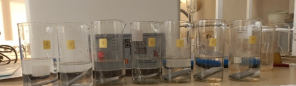
\includegraphics[width=\textwidth]{media/gor/image22}
    \end{subfigure}
    \begin{subfigure}{0.6\textwidth}
        \centering
        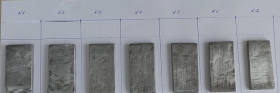
\includegraphics[width=\textwidth]{media/gor/image23}
    \end{subfigure}
    \caption*{1- сурет. Болат пластиналарын агрессивті ортаға салғанға дейінгі көрінісі}
\end{figure}

% \begin{figure}[H]
% 	\centering
% 	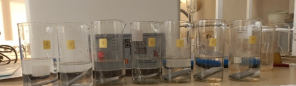
\includegraphics[width=0.8\textwidth]{media/gor/image22}
% 	\caption*{}
% \end{figure}


% \begin{figure}[H]
% 	\centering
% 	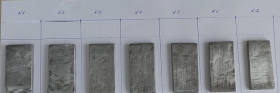
\includegraphics[width=0.8\textwidth]{media/gor/image23}
% 	\caption*{}
% \end{figure}


% {\bfseries 1- сурет. Болат пластиналарын агрессивті ортаға салғанға дейінгі
% көрінісі}

\begin{figure}[H]
    \centering
    \begin{subfigure}{0.6\textwidth}
        \centering
        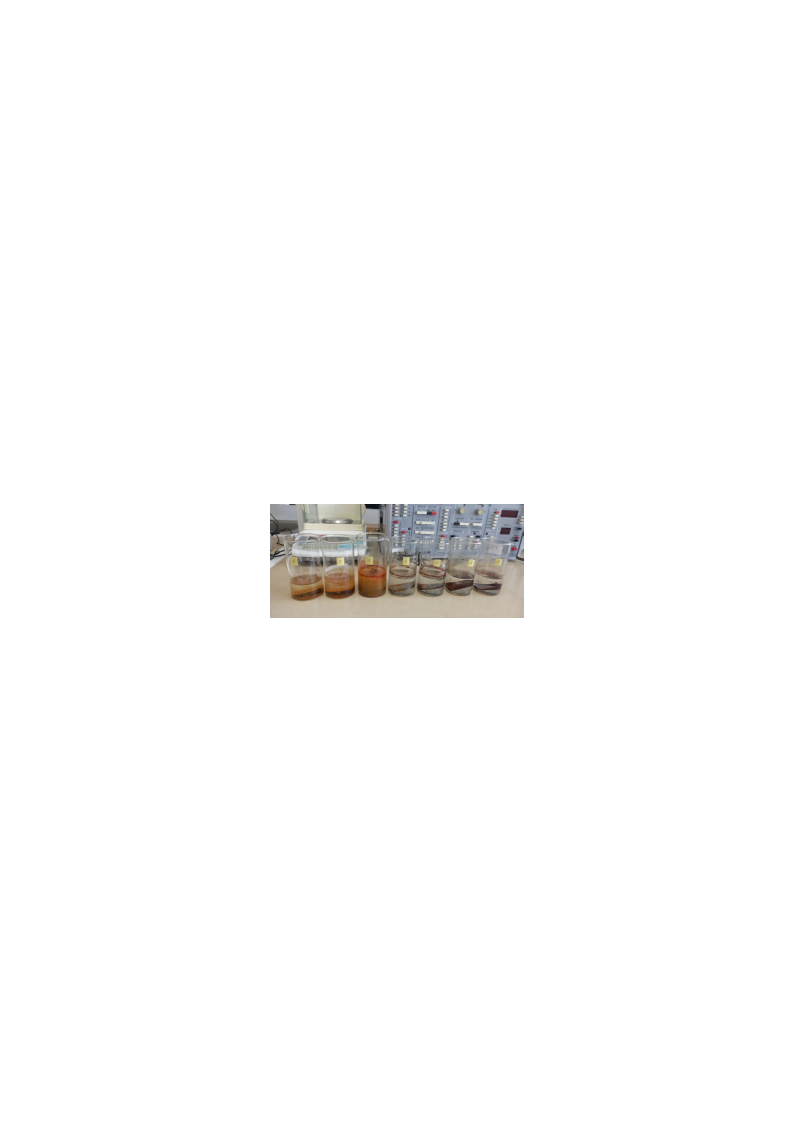
\includegraphics[width=\textwidth]{media/gor/image24}
        
    \end{subfigure}
    \begin{subfigure}{0.6\textwidth}
        \centering
        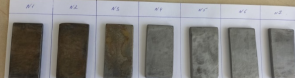
\includegraphics[width=\textwidth]{media/gor/image25}
        
    \end{subfigure}
    \begin{subfigure}{0.6\textwidth}
        \centering
        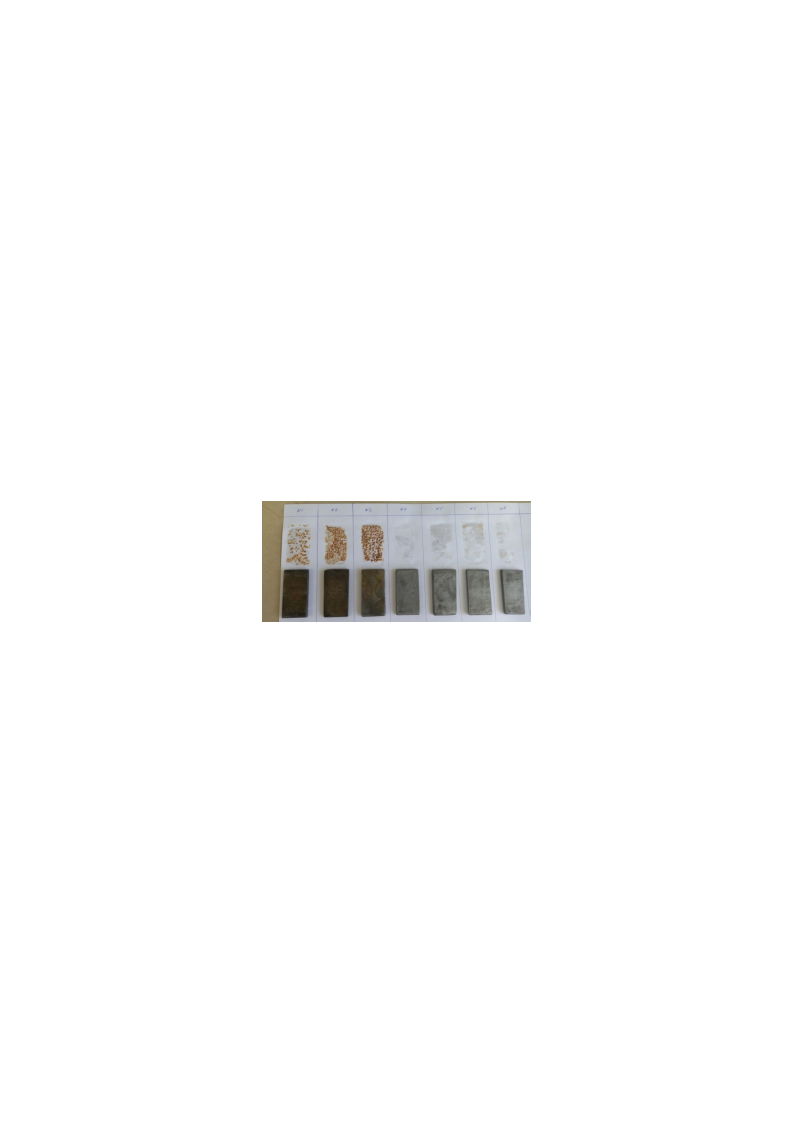
\includegraphics[width=\textwidth]{media/gor/image26}
       
    \end{subfigure}
    \caption*{2-сурет. Болат пластиналарының агрессивті ортада 15 тәулік ішінде коррозияға ұшырауының көрінісі}
\end{figure}

\begin{figure}[H]
	\caption*{ 1-кесте. Жануарлар майы негізіндегі реагенттерінің коррозияға
	қарсы қасиеттері}
	\centering
	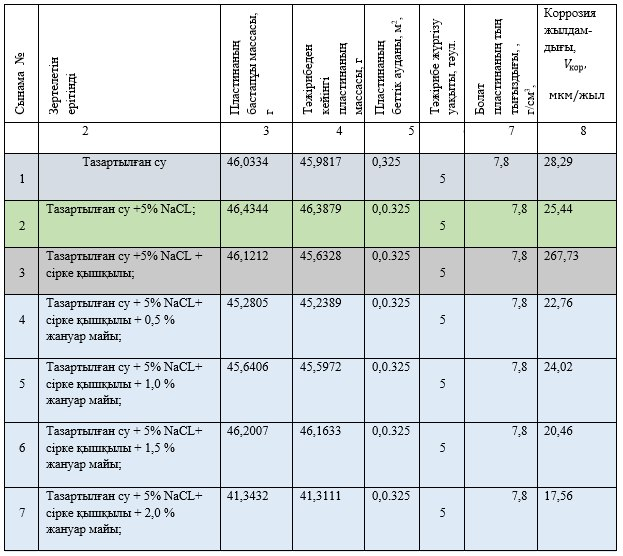
\includegraphics[width=\textwidth]{media/gor/image24.2}
	
\end{figure}



\begin{figure}[H]
	\centering
	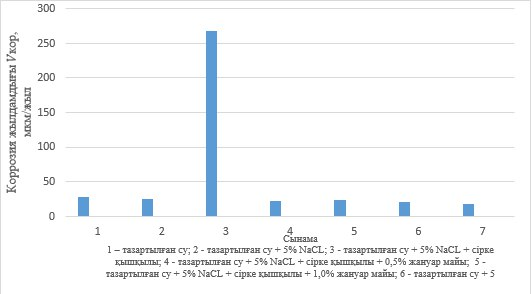
\includegraphics[width=0.6\textwidth]{media/gor/image24.5}
	\caption*{3 - сурет. Коррозия жылдамдығы, V\textsubscript{кор}, мкм/жыл }
\end{figure}

\begin{multicols}{2}



{\bfseries Қорытынды.} Жануарлар майының коррозияға қарсы қасиеттерін
тәжірибелік зерттеуде олардың болат пластиналар қабатында беттік
әрекеттік зат түзіп, пластиналар массасының жоғалуын төмендетіндігін
көрсетті. Осылайша, жануарлар майын экологиялық таза майлаушы қоспа
ретінде және бұрғылау құбырларының коррозияға қарсы қасиеттерін жақсарту
үшін пайдаланып қана қоймай, сонымен қатар оларды коррозиядан қорғау
мақсатында коррозия ингибиторы ретінде ұсынуға болады.
\end{multicols}


\begin{center}
	{\bfseries Әдебиеттер}
	\end{center}
	
	\begin{references}

1.Джаббаров Ш.Н. Современные проблемы коррозионной стойкости комплексов
подземного оборудования для добычи нефтепродуктов// Инновационные
технологии в науке и образовании: материалы VII Междунар. науч.-практ.
конф. ЦНС «Интерактив плюс» Чебоксары.- 2016.- № 3.- С.172-179. DOI
10.21661/r-112617

2. Ropus I., Cajner H., Curcovic L. Optimization of density of microwave
sinte ceramics due to the corrosion in nitric asid// 10 International
Conference «Mechanical Technologies and Structural Materials»// Split
Croatia, 2021.- P.139- 143. ISSN 1847-7917

3. Popoola L.T. Organic green corrosion inhibitors (OGCIs): A critical
review// Corr. Reviews.- 2019. - P.71-102. DOI 10.1515/corrrev-2018-0058

4. Козлов, В.А. Основы антикоррозионной защиты металлов: учеб.
пособие//Иван. Гос. хим.--технол. ун-т.-Иваново, 2014. -- с.177. ISBN
978-5-9616-0473-3

5. Roberge PR: Handbook of corrosion engineering. New York:
McGraw-Hill.- 2000.- 1139 p.

ISBN 0-07-076516-2

6. Oyelami B.O., Asere A.A. Mathematical modelling: An application to
corrosion in a petroleum industry. NMC Proceedings Workshop on
Environment. Abuja, Nigeria. National Mathematical Centre, 1999. - P.
48-66. https://www.researchgate.net/publication/252065867

7. Штырев О. О. Причины разрушения тела бурильных труб в процессе
эксплуатации и преимущества бурильных труб с внутренним защитным
покрытием//Территория Нефтегаз.- 2014.-№12.- С.90-92.

8. Perez T.E. Corrosion in the Oil and Gas Industry: An Increasing
Challenge for Materials // JOM.- 2013.- Vol.65(8) - P.1033-1042. DOI
10.1007/s11837-013-0675-3

9. Меркулов В.В., Акмалова И.М., Алмазов А.И., Ситдикова Е.В., Гавва
Н.Ф. Метод получения поверхностно-активных веществ на основе различного
жирового сырья// Международный журнал прикладных и фундаментальных
исследований. -- 2022. -- №12. -- С. 117-121. DOI 10.17513/mjpfi.13494

10.Mehdipour M., Ramezanzadeh B., Arman S.Y. Electrochemical noise
investigation of Aloe plant extract as green inhibitor on the corrosion
of stainless steel in 1~M H\textsubscript{2}SO\textsubscript{4}//
Journal of Industrial and Engineering Chemistry.- 2015.-Vol.21.-
P.~318-327.DOI \href{https://doi.org/10.1016/J.JIEC.2014.02.041}{10.1016/J.JIEC.2014.02.041}

\end{references}

\begin{center}
{\bfseries References}
\end{center}

\begin{references}
1.Dzhabbarov Sh.N. Sovremennye problemy korrozionnoj stojkosti
kompleksov podzemnogo oborudovanija dlja dobychi nefteproduktov//
Innovacionnye tehnologii v nauke i obrazovanii: materialy VII Mezhdunar.
nauch.-prakt. konf. CNS «Interaktiv pljus» Cheboksary.- 2016.- № 3.-
S.172-179. DOI 10.21661/r-112617. {[}in Russian{]}

2. Ropus I., Cajner H., Curcovic L. Optimization of density of microwave
sinte ceramics due to the corrosion in nitric asid// 10 International
Conference «Mechanical Technologies and Structural Materials»// Split
Croatia, 2021.- P.139- 143. ISSN 1847-7917

3. Popoola L.T. Organic green corrosion inhibitors (OGCIs): A critical
review// Corr. Reviews.- 2019. - P.71-102. DOI 10.1515/corrrev-2018-0058

4. Kozlov, V.A. Osnovy antikorrozionnoj zashhity metallov: ucheb.
posobie//Ivan. Gos. him.--tehnol. un-t.-Ivanovo, 2014. -- s.177. ISBN
978-5-9616-0473-3. {[}in Russian{]}

5. Roberge PR: Handbook of corrosion engineering. New York:
McGraw-Hill.- 2000.- 1139 p. ISBN 0-07-076516-2

6. Oyelami B.O., Asere A.A. Mathematical modelling: An application to
corrosion in a petroleum industry. NMC Proceedings Workshop on
Environment. Abuja, Nigeria. National Mathematical Centre, 1999. - P.
48-66. https://www.researchgate.net/publication/252065867

7. Shtyrev O. O. Prichiny razrushenija tela buril' nyh
trub v processe jekspluatacii i preimushhestva buril' nyh
trub s vnutrennim zashhitnym pokrytiem//Territorija Neftegaz.-
2014.-№12.- S.90-92. {[}in Russian{]}

8. Perez T.E. Corrosion in the Oil and Gas Industry: An Increasing
Challenge for Materials // JOM.- 2013.- Vol.65(8) - P.1033-1042. DOI
10.1007/s11837-013-0675-3

9. Merkulov V.V., Akmalova I.M., Almazov A.I., Sitdikova E.V., Gavva
N.F. Metod poluchenija \\poverhnostno-aktivnyh veshhestv na osnove
razlichnogo zhirovogo syr' ja// Mezhdunarodnyj zhurnal
\\prikladnyh i fundamental' nyh issledovanij. - 2022.-
№12.- S.117-121. DOI 10.17513/mjpfi.13494. {[}in Russian{]}

10.Mehdipour M., Ramezanzadeh B., Arman S.Y. Electrochemical noise
investigation of Aloe plant extract as green inhibitor on the corrosion
of stainless steel in 1~M H\textsubscript{2}SO\textsubscript{4}//
Journal of Industrial and Engineering Chemistry.- 2015.-Vol.21.-
P.~318-327.
DOI \href{https://doi.org/10.1016/J.JIEC.2014.02.041}{10.1016/J.JIEC.2014.02.041}
\end{references}

\begin{authorinfo}
\hspace{1em}\emph{{\bfseries Авторлар туралы мәлімет}}

Охапова К.Т.- докторант, М.Әуезов атындағы Оңтүстік Қазақстан
университеті, Шымкент қ., Қазақстан,\\e-mail: nuri.maksim82@mail.ru;

Шуханова Ж. К.- PhD, М. Әуезов атындағы Оңтүстік Қазақстан университеті,
Шымкент қ., Қазақстан, \\e-mail: shuhanovaz@mail.ru;

Бондаренко В.П.-техника ғылымдарының кандидаты, доцент, М. Әуезов
атындағы Оңтүстік Қазақстан университеті, Шымкент қ., Қазақстан, e-mail;

Сагитова Г. Ф.- техника ғылымдарының кандидаты, профессор, М. Әуезов
атындағы Оңтүстік Қазақстан университеті, Шымкент қ., Қазақстан, e-mail:
guzalita.f1978@mail.ru.

\hspace{1em}\emph{{\bfseries Information about the author}}

K. Okhapova- PhD student, M. Auezov South Kazakhstan university,
Shymkent,Kazakhstan, e mail: nuri.maksim82@mail.ru;

Zh. Shukhanova -- PhD, docent, M. Auezov South Kazakhstan university,
Shymkent, Kazakhstan, e-mail: shuhanovaz@mail.ru;

V.Bondarenko - Candidate of technical sciences, Assoc.professor M.
Auezov South Kazakhstan university, Shymkent, Kazakhstan, e mail:
vbond2011@mail.ru;

G. Sagitova - Candidate of technical sciences, professor ,M. Auezov
South Kazakhstan university, Shymkent, Kazakhstan; e mail:
guzalita.f1978@mail.ru.
\end{authorinfo}
